\documentclass[journal]{IEEEtran}

\usepackage{graphicx}
\usepackage{hyperref}

\hypersetup{
    colorlinks=true,
    linkcolor=black,
    filecolor=black,      
    urlcolor=cyan,
    pdftitle={Computer Vision Chessboard},
    pdfpagemode=FullScreen,
    }

\usepackage[style=numeric]{biblatex}

\addbibresource{references.bib}

\newcommand\mkbibcolor[2]{\textcolor{#1}{\hypersetup{citecolor=#1}#2}}
\DeclareCiteCommand{\cite}[\mkbibcolor{black}]
  {\usebibmacro{prenote}}%
  {\usebibmacro{citeindex}%
   \usebibmacro{cite}}
  {\multicitedelim}
  {\usebibmacro{postnote}}

\begin{document}

% paper title
% can use linebreaks \\ within to get better formatting as desired
\title{Computer Vision Chessboard}

\author{Brandon~LeMay}

% make the title area
\maketitle

% As a general rule, do not put math, special symbols or citations
% in the abstract or keywords.
\begin{abstract}
A computer vision enable chessboard was built to track chess pieces throughout a chess match. External chess engines were used to suggest moves to the user, or play against a computer using a physical chessboard. The current chess position is reflected virtually on a touchscreen interface, with a custom PCB control board providing the interface for the user to manage execution of chess tracking program. The program can track an entire chess game successfully, as well as adapt the skill of the chess engine to suit the user's preference. This sets up a platform allowing a computer to physically play chess against a human by replicating the ability of a human to track changes in a chessboard, in addition to implementing object detection functions that can be applied to tracking objects of any known color and shape in known sections of an image.
\end{abstract}

\begin{IEEEkeywords}
Chess, Computer Vision, OpenCV, Apriltag, Raspberry Pi.
\end{IEEEkeywords}


\section{Introduction}
\IEEEPARstart{C}{hessboards} as the subject of computer vision experiments are certainly nothing new. Blank chessboards are widely studied in computer vision both as methods to calibrate cameras, as chessboards have a very predictable geometry, so lens distortions are easy to counteract, and as a classic example for feature extraction, where a computer attempts to identify the distinct edges and corners of a chessboard in an image. [\cite{Forsyth2002}]

Many projects have also addressed the additional challenges of using computer vision to analyze a picture of a chessboard and return the types and positions of each piece on the board. Being able to determine the position of all chess pieces on a given board simply from a photo or video helps tremendously in incorporating chess engines in physical products, and the image processing functions for detecting objects based on shape and color from multiple perspectives with varying levels of obstruction can be applied in countless scenarios. Most of projects focusing on chess vision focus on taking a single image and converting it to a board layout that shows which pieces occupy each square.

Some projects identify the location of a chessboard pattern in a picture and use a neural network to identify the location, color, and type of piece on each square [\cite{Czyzewski2018}], or use a pretrained neural network to identify piece type [\cite{Saurabh2019}].

The most relevant work to this project was a Masters Thesis done by Zoltán Orémuš that computes chess position from a single photo with no machine learning, only image processing. [\cite{Orémuš2018}] Major differences between this project and his algorithm are that this project uses fiducials to localize the chessboard, and this project needs no prior knowledge of piece geometry or height.

Instead of focusing on capturing the the position of a chessboard from a single photo, this project aims to tell the position of a chessboard given an unbroken stream of photos starting at the beginning of a match. By tracking the position of each piece as each move is made, the complexity of the image processing required to obtain a full chess position. For each new frame that needs to be processed, one can use the knowledge of where pieces were in the past frame, rendering the problem of being able to differentiate piece types irrelevant. Because each piece is tracked as it moves from square to square, and each piece starts in a known square, the program can keep track of the type of each piece as it moves.

To keep this project small enough to be able to accomplish in one semester, several assumptions were made, including being able to customize the chessboard to have fiducials in each corner, and a custom pattern around the edge to assist in image processing of the chessboard. In addition, the color detection method was adapted specifically for the silver and gold pieces used with this chessboard.

Some of the most important issues solved to be able to track pieces throughout a chess match were being able to determine how thresholds should be set to work in multiple lighting conditions, and how to tell when a user or any other obstruction is blocking the camera's view of the chessboard.

To accomplish the task of tracking chess pieces throughout a chess match, a custom chessboard was manufactured with tags and patterns to aid in image processing, and a camera was suspended above the chessboard with controllable LEDs lighting the chessboard. A chess tracking program was written in Python, using OpenCV, among other libraries, to continuously take images of the chessboard and compute the location and color of each piece on the board. These functions could easily be applied to tracking other objects that exist in known sections of a image.

\section{Analysis of Applicable Standards}
This project does not comply with IEEE Standard for Software Test Documentation (IEEE Std 829-1998), largely due to the absence of recorded test logs. Tests performed on the software either have no record stored anywhere of the execution or results of the test, with the only consequence of the test being that the code was modified to better adapt to the test environment.

This project does however comply with IEEE Standard for Software User Documentation (IEEE Std 1063-2001). Each function of the Python program has a multiline description of the purpose and use of the function, as well as inline comments describing the purpose of each line or group of lines. In addition, labeled illustrations are provided, including ideal pictures of each stage of the image processing, as well as a flowchart of the flow of the program.

It should also be noted that the power supply used for powering the chessboard is certified by the Underwriters Laboratories.

\section{Work}
The computer vision program for monitoring the chessboard runs on a Raspberry Pi embedded in the frame of the chessboard. The program was written in Python, and can be split in three discrete sections: frame processing, where a picture of the chessboard is taken and analyzed to determine the position and color of each piece on the board. This information is then passed to the second section of the code that compares the current state of the board to the last state, and returns the move that was made to change the state of the board, if any. Lastly, another section of the code deals with peripherals meant to improve the user experience of the chessboard, including an animated representation of what the computer sees as the current board, and a custom PCB to control the chessboard, with buttons for starting, pausing, and stopping a game, as well as offering a draw or resigning.

\subsection{Physical Components and Construction}
A variety of manufacturing methods were used to create the physical chessboard, including milling, 3D printing, laser cutting, waterjet cutting, and sheet metal folding. The CAD model of the completed chessboard can be seen in Figure \ref{render}.


\begin{figure}[!ht]
	\centering
	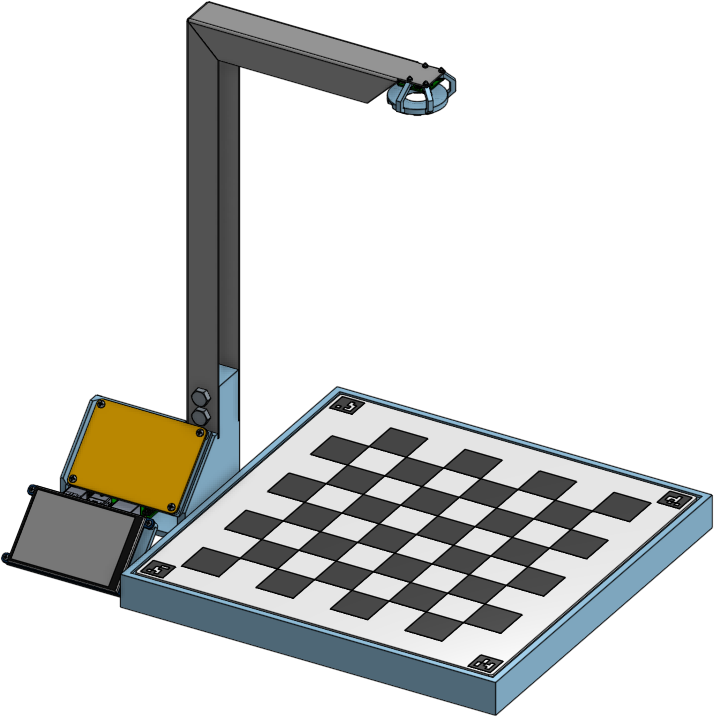
\includegraphics[width=\linewidth]{Images/Render.png}
	\caption{3D Render of CAD Model}
	\label{render}
\end{figure}

\vspace{12pt}

\subsubsection{PCB Milling}
A custom PCB was designed using EAGLE. The purpose of this circuit board is to provide a user interface that doesn't require a mouse or keyboard. A number of inputs were added to this PCB to communicate with the Raspberry Pi, including 5 buttons: 1 to start or pause a chess match, 1 to stop an ongoing match, 1 to toggle whether the user plays as white or black, 1 button for requesting a hint from a chess engine, and 1 button for offering a draw.

Figure \ref{PCB} shows the board design, the PCB has 2 copper layers, the red traces show the top layer, and blue denotes the bottom layer. Keen observers will note there is blue in the image than there is red, the bottom layer has a ground plane, so any "extra" copper not used for traces is connected to 0V.
The full PCB design files can be found in the repository linked in Appendix \ref{Github repo}.

\begin{figure}[!ht]
	\centering
	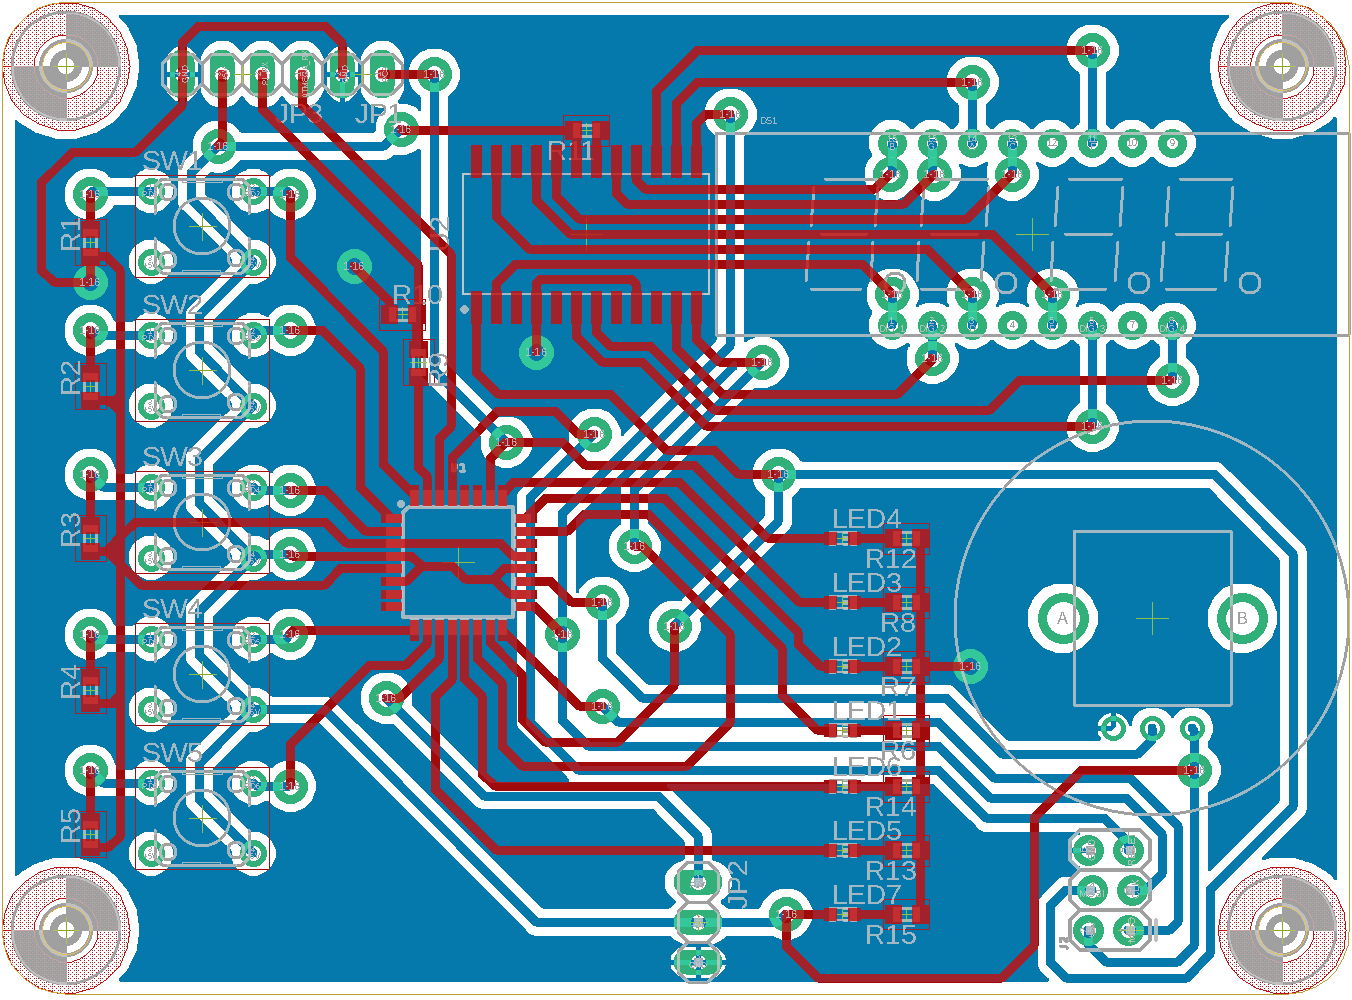
\includegraphics[width=\linewidth]{Images/ControlBoardDesign.png}
	\caption{Full Layer Stack of Control Board}
	\label{PCB}
\end{figure}

Also included are 6 controllable LEDs: 1 displays whether the user is playing as white or black, and the other 5 for signaling errors.
There is also another LED that automatially powers on when the circuit board is powered, this provides an easy way for the user to tell when the chessboard is powered.

To switch between the user playing another person and playing a computer, as well as selecting the skill of the computer, a potentiometer was added to the control board. The potentiometer has a detent in the middle of rotation, potentiometer positions to the counter-clockwise of the detent are for the user playing another human, with the position determining the skill of the chess engine providing hints. When the potentiometer is positioned on the detent, the chess engine is disabled and only move tracking is enabled for a more natural playing experience. When the potentiometer is positioned clockwise of the detent, the user plays against a chess engine, the rating of which is detemined by how clockwise the position is, more clockwise positions increase the skill of the chess engine.

Directly above the potentiometer is a 7-segment display that shows the rating of the chess engine, detemined by the potentiometer position. During gameplay, the display shows the move selected by the chess engine.

Lastly, three connectors are included on the board, one to power and control the LED ring around the camera that lights the chessboard, one to interface with the Raspberry Pi, and one to enable programming of the microcontroller on the PCB.

%\begin{figure}[!ht]
%	\centering
%	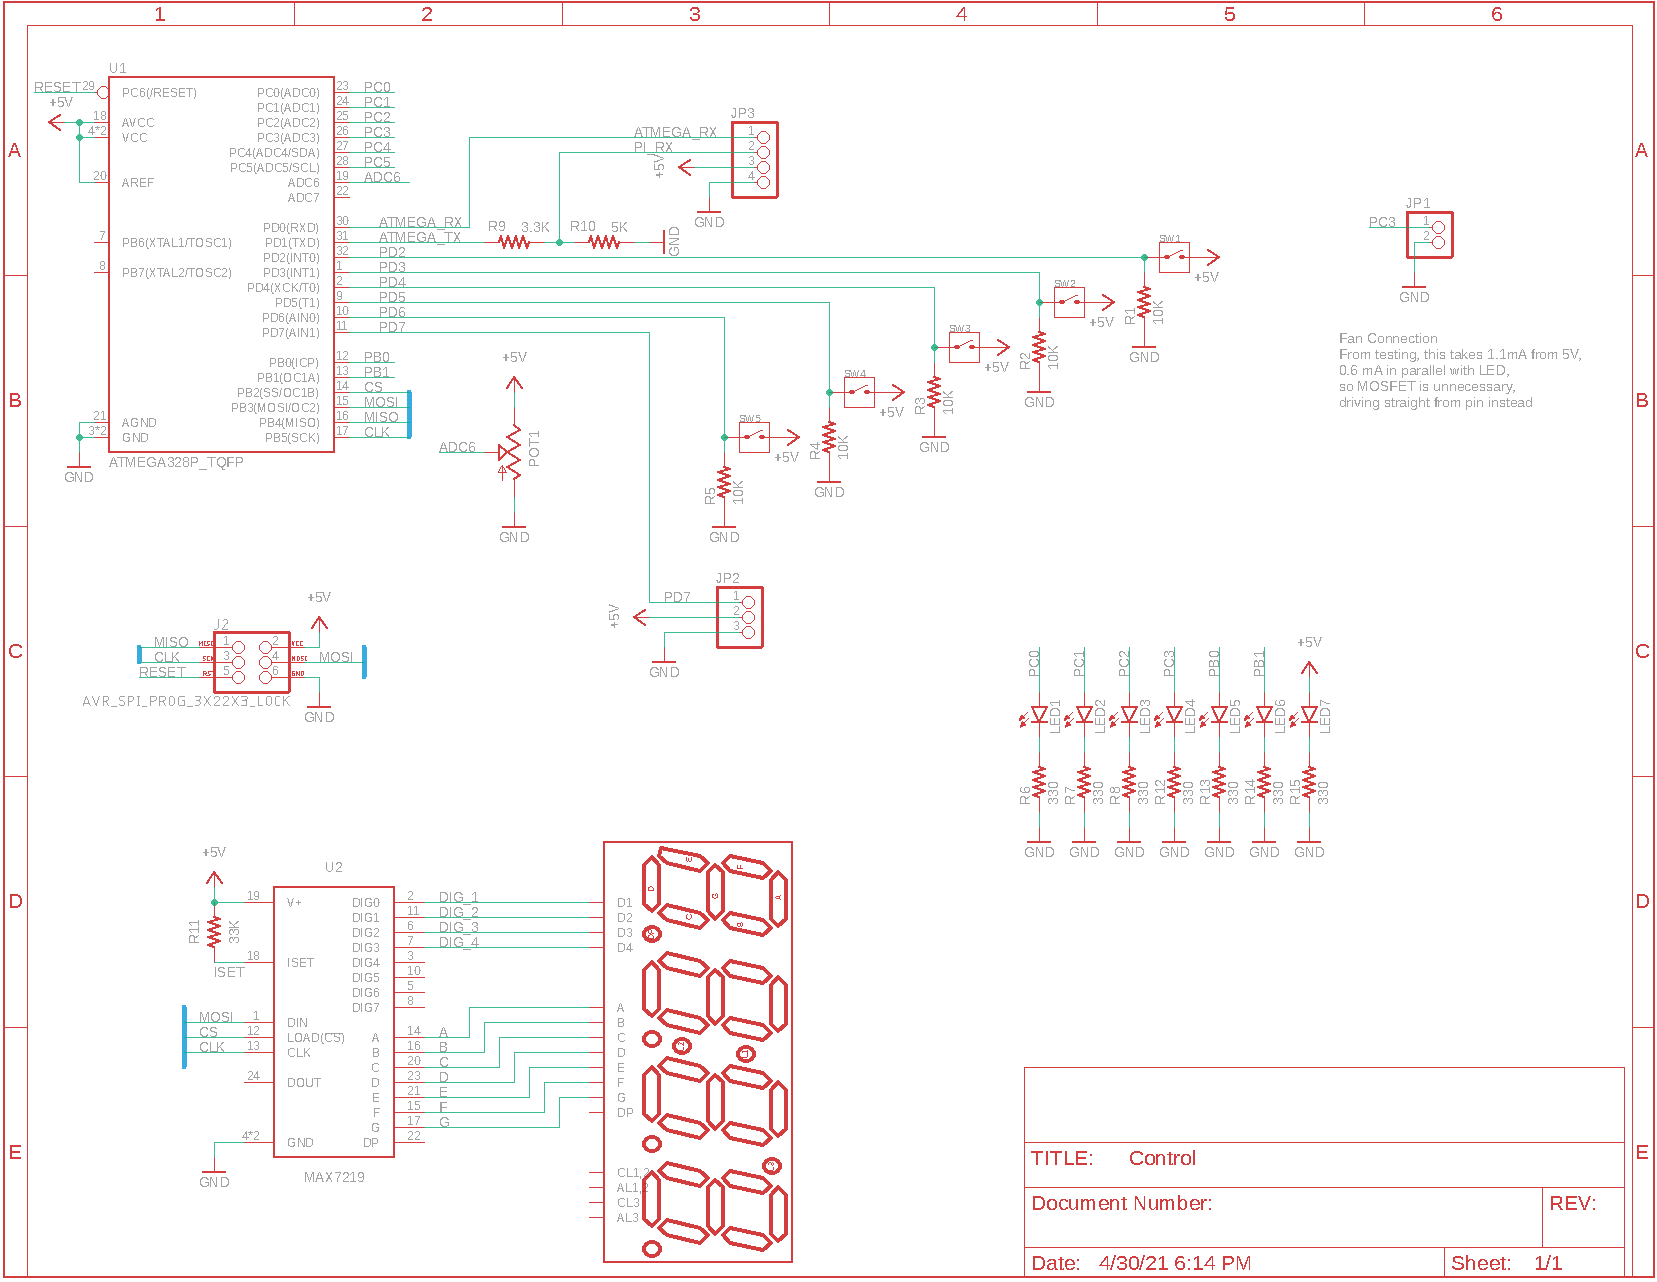
\includegraphics[width=\linewidth]{Images/ControlSchematicDesign.png}
%	\caption{Full Layer Stack of PCB}
%	\label{render}
%\end{figure}

To manufacture the circuit board, Gerber files were generated from the EAGLE design, which were then cut on an LPKF circuit board milling machine. A brass solder stencil was milled on an Othermill, and then used to apply solder paste to the pads of all the surface mounted devices (SMD). The SMD components were then placed on the board with tweezers, and the assembly was placed in a reflow oven to solder all SMD joints at once. Lastly, the remaining through-hole mounted (THM) components were placed and soldered by hand.

To program the ATMega328p on the circuit board that reads inputs from the buttons and potentiometers, communicates with the Raspberry Pi, and sets the display of the 7-segment display and LED ring, an AVR programmer was used. The code was written in C, compiled with avr-gcc, and written to the microcontroller using avrdude and a USBTiny ISP programmer

\vspace{12pt}

\subsubsection{3D Printing}
To compactly mount the Raspberry Pi, control PCB, and touchscreen display, and have user oriented components angled towards the user, exotic geometry was required. To easily fabricate these complex shapes, a Prusa MK3S FFM 3D printer was used.

Two important parts of the chessboard were 3D printed: the chessboard base that holds all the chess pieces when not in use and the chessboard sits on top of, and which the Raspberry Pi, control PCB, and touchscreen display all mount on. This base can be seen in Figure \ref{BoardMount}. 

\begin{figure}[!ht]
	\centering
	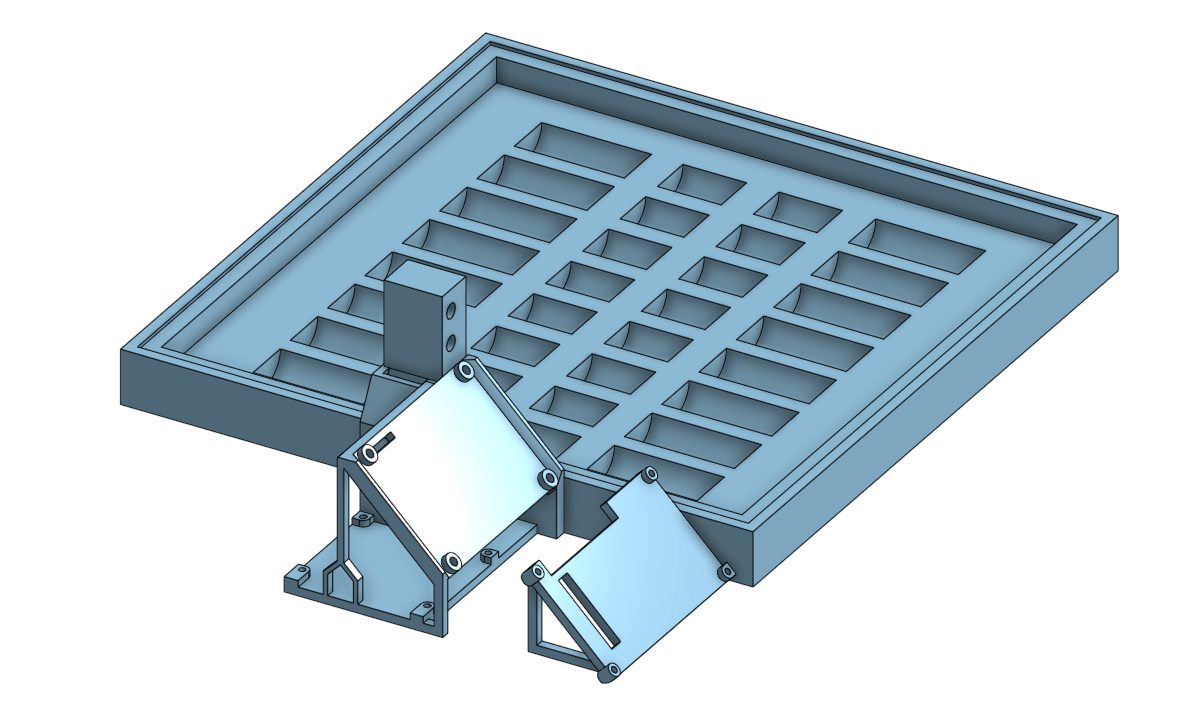
\includegraphics[width=\linewidth]{Images/BoardMount.png}
	\caption{Chessboard Base}
	\label{BoardMount}
\end{figure}

In addition, the LED light ring used to illuminate the chessboard is mounted to a 3D printed part that suspends it just below the camera to prevent it from blocking the cameras view while giving the light an unobstructed path to light up the chessboard. This standoff can be seen in Figure \ref{LEDMount}. 

\begin{figure}[!ht]
	\centering
	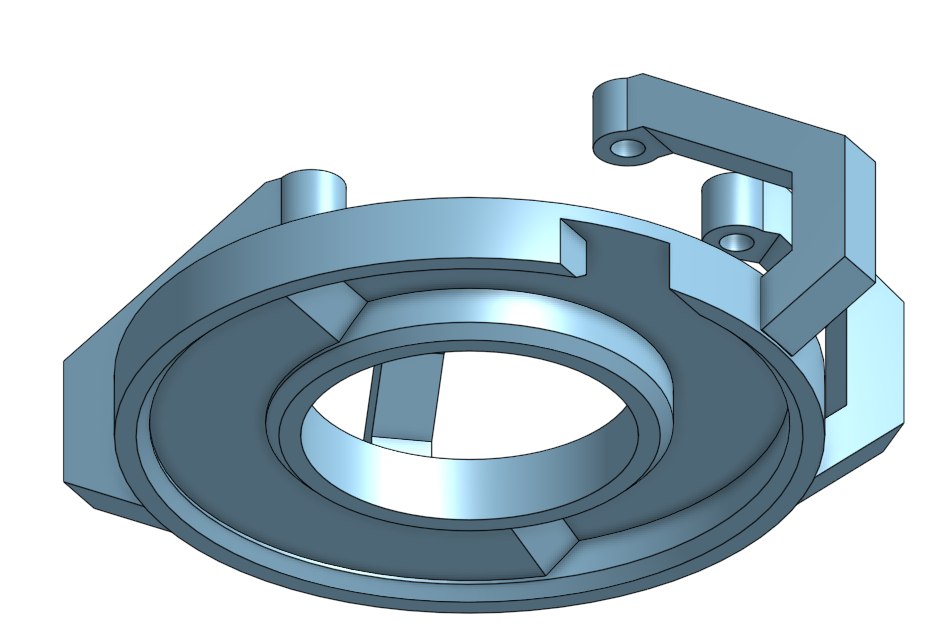
\includegraphics[width=\linewidth]{Images/LEDMount.png}
	\caption{LED Ring Light Mount}
	\label{LEDMount}
\end{figure}

The arms stretching above the circle set the mount just below the camera, while cutouts in the circle allow for wires to be soldered to the back of the LED ring and easily routed.

\vspace{12pt}

\subsubsection{Laser Cutting}

The wooden chessboard upon which the game is played was laser cut out of birch plywood, the interior of the board has the classic alternating pattern of colored squares that pieces are placed on, while the border of the board was reserved for image processing features. Apriltag fiducials were placed on each corner to assist in locating the chessboard in the frame of any image. Section \ref{ApriltagDetection} gives more information on this process. In between each tag, a Celtic knot pattern was placed, this design is used to tell when a user places their hand above the chessboard and obstructs the camera view. This feature is discussed more in Section \ref{ApriltagDetection}.

Figures \ref{input} and \ref{KnotCrop} show the chessboard from the perspective of the Raspberry Pi camera.

\vspace{12pt}

\subsubsection{Sheet Metal Forming}
To hold the camera above the chessboard, a crane was cut from aluminum sheet metal. Metal was used instead of plastic because the part was easily manufactured from flat panels, and provides more strength and rigidity, which is important to minimize blurring in images of the chessboard from the camera bouncing and flexing at the edge of the crane.

To make this part, the pattern shown in Figure \ref{CraneFlat} was cut on a waterjet cutter.

\begin{figure}[!ht]
	\centering
	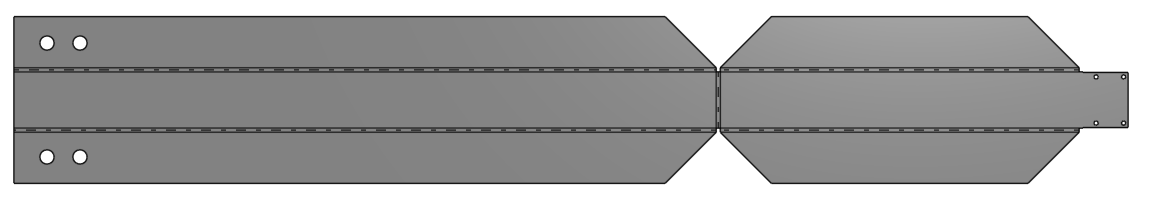
\includegraphics[width=\linewidth]{Images/CameraCraneFlat.png}
	\caption{Sheet Metal Crane Flat Pattern}
	\label{CraneFlat}
\end{figure}

This part was then folded on a sheet metal brake to form the shape shown in Figure \ref{Crane}.

\begin{figure}[!ht]
	\centering
	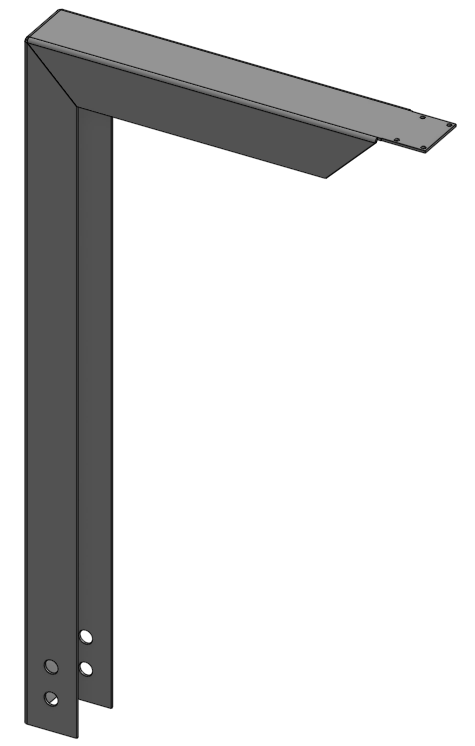
\includegraphics[width=0.7\linewidth]{Images/CameraCrane.png}
	\caption{Folded Sheet Metal Camera Crane}
	\label{Crane}
\end{figure}

This sheet metal crane fastens to the board mount shown in Figure \ref{BoardMount} using two large bolts, and the camera and LED ring mount onto the end of the crane using 4 M2.5 screws.

\vspace{12pt}

\subsection{Frame Processing}
The image processing component of the move tracking software can be split further into 4 sections: chessboard localization and cropping, obstruction testing, piece detection, and color detection. 

The program was designed with the assumption that the chessboard will not be in a fixed position in relation to the camera, and thus the first step for processing any frame is to find the location of the chessboard in the frame. Once the chessboard has been found, the corners of the chessboard are used to transform the image such that the rows and columns of the chessboard are horizontal and vertical in the frame of the image. As part of this transform, any area of the frame outside the chessboard is cropped.

After the chessboard has been located and transformed, the pattern on the edges of the board are compared to a template to make sure there is nothing obstructing the view of the chessboard from the camera. If any significant portion of the pattern is missing, then it is likely that a hand or arm is in the frame moving a piece, so the frame is thrown out and a new frame is taken.

Assuming no obstructions are detected, the frame is split into individual squares. These squares are then run through an edge detection algorithm to detect the amount of edges (sharp variations in color among nearly pixels) in the square. If the number of edges in a given square exceeds a certain threshold, the square is labelled as occupied.

Once each square has been labelled occupied or empty, the occupied squares are run through a color detecting function that converts the RGB image to HSV and uses the hue values of the square to determine what color the piece is, and thus can decide what side the piece belongs to.

Finally, an array containing both which squares are occupied and what color each of the pieces in an occupied square are is sent to the set of functions that parses what move was made, if any.

Figure \ref{input} shows an example of an input image. All the pieces are in their starting positions, and the edges of the chessboard are clearly visible, with no hands or arms reaching over the board to manipulate any pieces, thus this image should be processed as a valid image. This is the same input image used to derive most other images in this report, any visualizations not using this input image to start will be explicitly noted.

\begin{figure}[!ht]
	\centering
	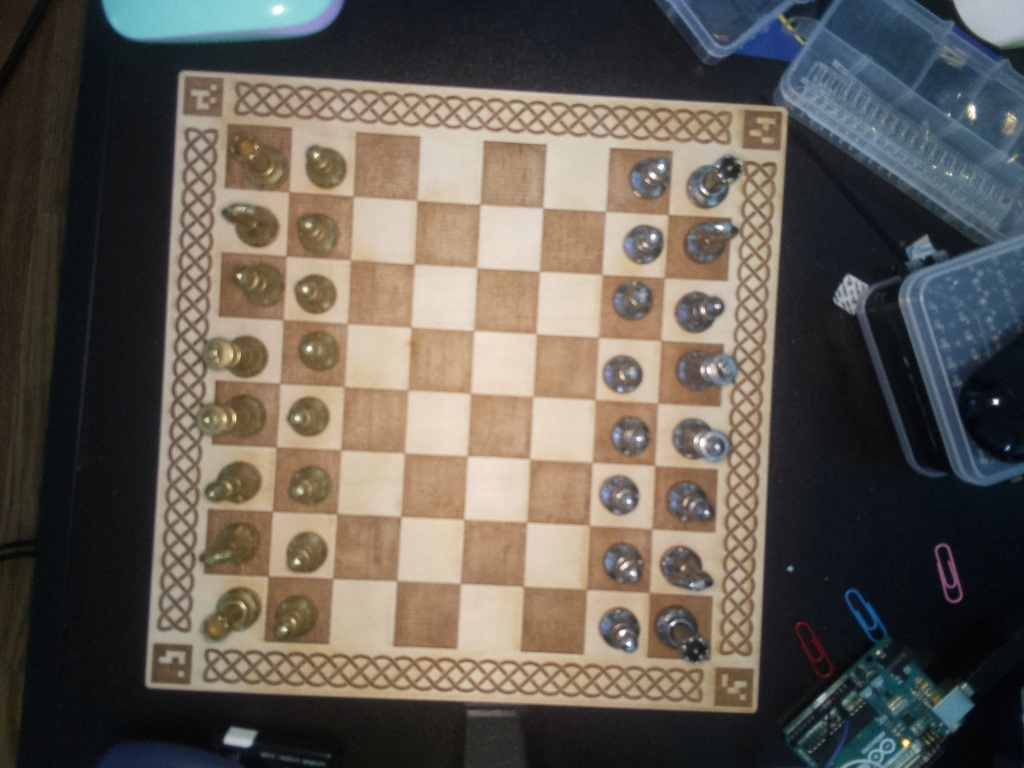
\includegraphics[width=\linewidth]{Images/InputImage.jpg}
	\caption{Input Image}
	\label{input}
\end{figure}

\vspace{12pt}

\subsubsection{Chessboard Localization}
\label{ApriltagDetection}
To determine where the chessboard is in the input frame, Apriltags were placed in each corner of the chessboard. Apriltags are a collection of unique two-dimensional patterns that can be easily detected using a camera, similar to a QR code, but much simpler in design to be easily recognized from a variety of distances [\cite{Wang2016}]. Each corner has an Apriltag with a different ID, which is recognizable by the computer when processing the image, thus the orientation of the chessboard can be kept constant.

To detect the Apriltags in the image, the python Apriltag library was used.
The tag detection was a significant bottleneck for the speed of the program, as the Raspberry Pi needs to determine the position of the chessboard in every frame, so running tag detection for every frame slowed down the processing time for each frame. To search the entire image for Apriltags took 762.9 milliseconds, in comparison, the rest of the image processing took a maximum of 500 seconds, so this delay in processing was significant.
%Check that processing time for the rest of the program
To decrease the time it takes to locate the chessboard, after the first frame is processed as normal, subsequent frames only search a small rectangle around where the tag was located in the previous frame. The time to find one Apriltag in one of these cropped search areas was 2.8 milliseconds, so the time to locate the chessboard was reduced to roughly 12 milliseconds, 63 times faster.

If the Apriltag detection algorithm returns a set of tags that doesn't contain the tags on the corners of the chessboard, the frame is ignored and another picture is taken to reexamine. The most likely reason for a tag not being included in the set of detected tags is because something is blocking the tag, so if there is an obstruction over any corner of the chessboard the frame can be thrown out without having to specifically test for any obstructions.

In order to be certain the Apriltags on the chessboard can be detected by the camera, the 16h5 tag family was chosen. This family of tags are all 4 pixel squares, the lowest amount of pixels per tag of any Apriltag family, allowing for each pixel to be larger than any other tag, meaning the tag is more likely to be detected.
This also means that it is easier for the Apriltag detection algorithm to return false positives, since each tag has less detail and thus non-tag objects or camera artifacts can appear to be valid tags by total chance. To remove these from consideration, the only detected tags that are used are tags that match the tag ID of the tags placed on the chessboard, and from those tags, only the 4 with the highest confidence are kept. Part of the information returned by the Apriltag detection algorithm is the confidence value for the tag, very clear tags have high confidence values, partially obstructed or blurry tags have low confidence values, thus by only keeping the tags with the 4 best confidence values, false positives are eliminated.

\vspace{12pt}

\subsubsection{Obstruction Testing}
\label{KnotDetection}

Once all 4 tags have been detected, the outside corners of the tags are used to reorient the perspective of the image. To do this, the image is transformed such that the pixel location representing the outside corner of each tag becomes the new corner of the image. Since the tags are equally spaced in each corner, this means that the horizontal rows of the chessboard are horizontal in the image, and the vertical columns are also vertical in the image. The outside corners are used to reorient the image so that the pattern going around the edges of the chessboard is visible, as can be seen in Figure \ref{KnotCrop}. 

\begin{figure}[!ht]
	\centering
	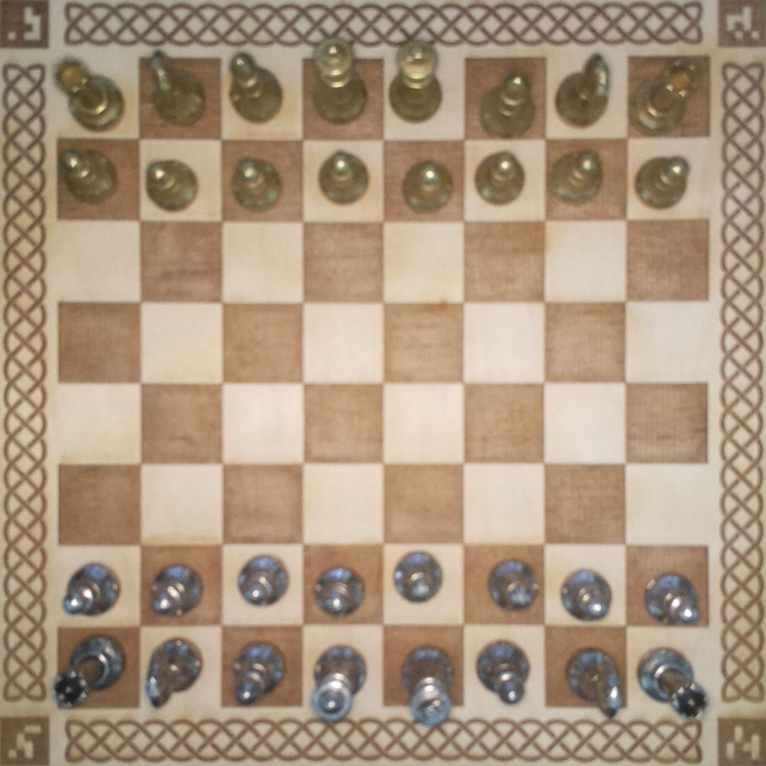
\includegraphics[width=\linewidth]{Images/InputImage_KnotCrop.jpg}
	\caption{Perspective Shifted Image}
	\label{KnotCrop}
\end{figure}

This knot pattern is used for testing whether a frame has an obstruction in it. For example, images where the user is moving a piece can't be used for image processing since the user's hand blocks the view of the camera. 
To detect whether this is the case, the detected edge pattern is compared to the pattern that was engraved onto the board.
This comparison is done by first scaling the template against which the detected pattern is to be compared to be the same size as the input image. Then, Canny edge detection is run on just the borders of the chessboard, excluding the inside of the board where all the squares are, as well as the corners of the board where the Apriltags are engraved.
The edges returned by the edge detection algorithm are then blurred to ensure that the pixels returned by the edge detection algorithm spread past just the edges of the pattern to fill the inside of each line.
An example of how this looks is given in Figure \ref{knot}, where these calculations are overlayed on the input image.

\begin{figure}[!ht]
	\centering
	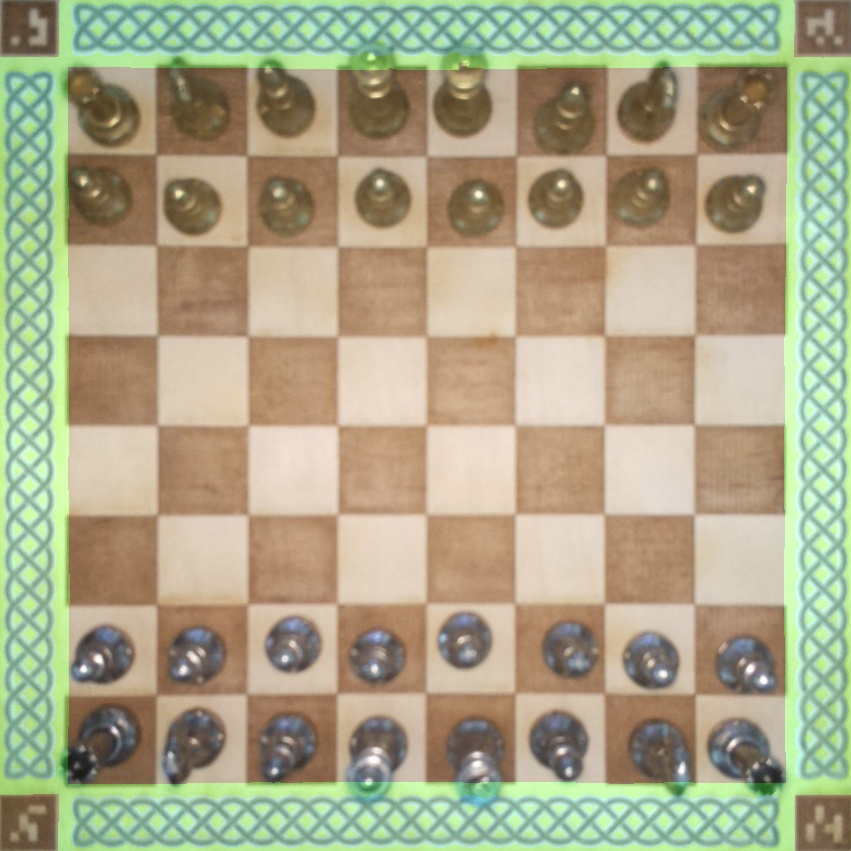
\includegraphics[width=\linewidth]{Images/KnotDetection.jpg}
	\caption{Obstruction Detection}
	\label{knot}
\end{figure}

The green blobs covering each edge are the blurred edge results, while the template to compare to are shown in blue.
Note that the blurring also acts to cover up small gaps missing from the pattern. In Figure \ref{knot} it is obvious to a human viewer that nothing is obstructing the camera's view of the chessboard, but close examination of the edge pattern would reveal small gaps where the perspective causes the king and queen pieces of both sides to cover up small portions of the pattern. But because the edge detection pixels are blurred, these small gaps are covered in green, which signifies that that portion of the pattern is considered accounted for.

To determine if there is an obstruction, the blurred edge matrix is subtracted from the template matrix. If the edges covers all portions of the template, this subtraction will result in zeros in every postition of the matrix. Any positive elements of the matrix are locations where the blurred edges don't cover the template. This implies that positive elements in the matrix resulting from taking the difference between the template and the blurred edges show areas where the camera is being obstructed.

This can be seen in Figure \ref{knot error}, where the green pixels again show the blurred edge matrix, and the template pattern is shown in blue, but any positive values of the difference matrix are shown in red.

\begin{figure}[!ht]
	\centering
	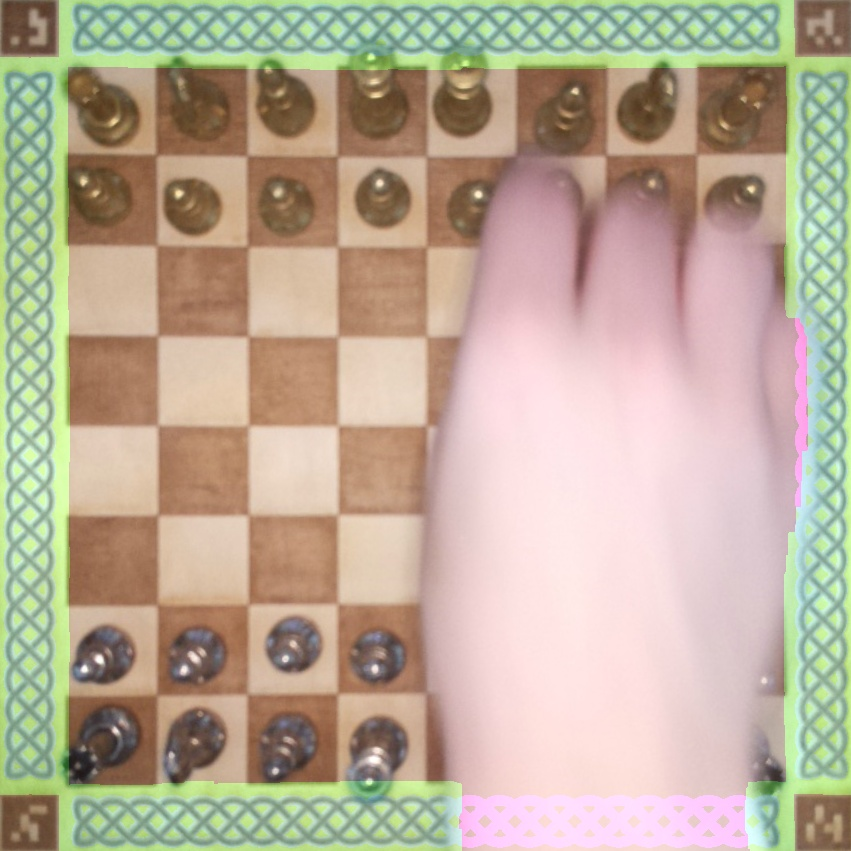
\includegraphics[width=\linewidth]{Images/KnotDetectionError.jpg}
	\caption{Obstruction Detection Error}
	\label{knot error}
\end{figure}

It is clear here that the wrist and the pinky both obstruct the edges of the chessboard, thus this image wouldn't be used image processing and another frame would be taken instead.

\vspace{12pt}

\subsubsection{Piece Detection}
\label{PieceDetection}
Once the chessboard has been located and tested for obstructions, the program moves on to detecting where pieces are located on the chessboard.
Since pieces should be located within the bounds of each square of the chessboard, the first step in detecting the pieces is to split up the input image into individual squares.

To divide the image, first the image is cropped to get rid of the borders of the chessboard and just focus on the squares. To do this, the image is transformed such that the inside corners of each Apriltag becomes the corners of the image.
The perspective shifted image can be seen in Figure \ref{InsideCrop}.

\begin{figure}[!ht]
	\centering
	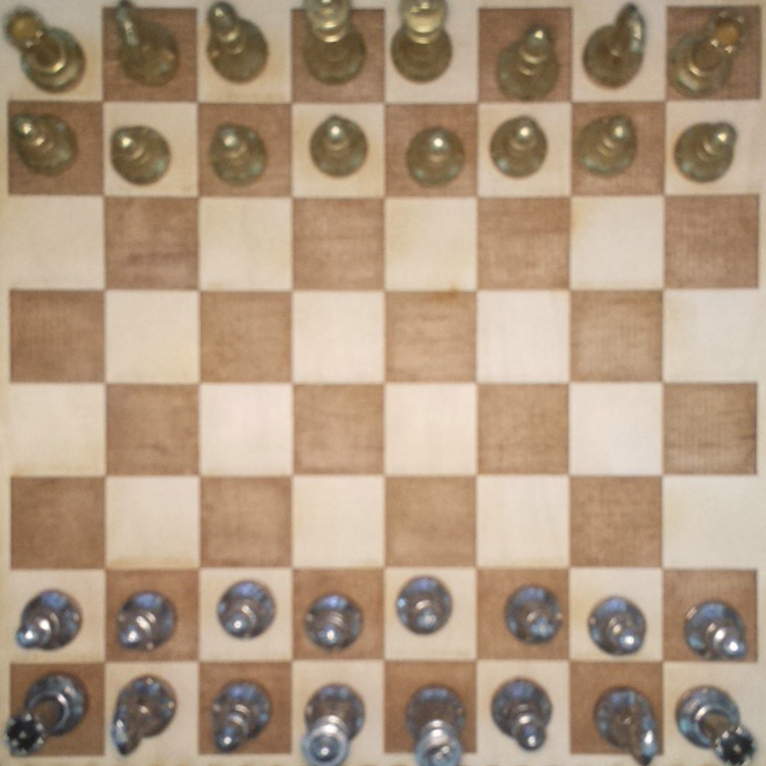
\includegraphics[width=\linewidth]{Images/InputImage_InsideCrop.jpg}
	\caption{Perspective Shifted Chessboard}
	\label{InsideCrop}
\end{figure}

The squares that are examined to determine if the square on the chessboard is occupied by a piece are all slightly smaller than the area of the square on the chessboard to create a border at the edge of each square that isn't used for piece detection. This border allows for pieces to be poorly placed or overlapping other squares without affecting the piece detection of nearby squares.

Figure \ref{piece zoomed} shows an example square of a populated square.

\begin{figure}[!ht]
	\centering
	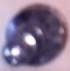
\includegraphics[width=\linewidth]{Images/KnotDetection340Zoomed.jpg}
	\caption{Single Occupied Square}
	\label{piece zoomed}
\end{figure}

The general idea to tell if a square is populated or not is to run Canny edge detection on the image of the square, then sum the number of edges detected. Figure \ref{piece detection zoomed} shows the result of Canny edge detection run on Figure \ref{piece zoomed}. The edge detection algorithm returns an array of ones and zeros, the zeros are shown as black pixels, and represent pixels from the original image that are not edges. The ones in the array are shown as white pixels, and represent pixels from the original image that are deemed edges.

\begin{figure}[!ht]
	\centering
	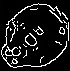
\includegraphics[width=\linewidth]{Images/PieceDetection340Zoomed.jpg}
	\caption{Single Square Piece Detection}
	\label{piece detection zoomed}
\end{figure}

If the total edge count of a square is greater than a predetermined threshold, then the square is deemed to be populated. The comparison threshold is automatically set from the data gathered in the first frame taken by the program. It assumes that the pieces will be in the starting position, and uses the average number of edges detected in the front and back two rows, where all the pieces start, to determine the average edge count of a populated square. The comparison threshold is then set to half the average value to account for lighting differences that might result in a piece blending in better with the board and returning less edges then average.

To help debug or diagnose errors, the program assembles all the single square images into the image shown in Figure \ref{piece detection}.

\begin{figure}[!ht]
	\centering
	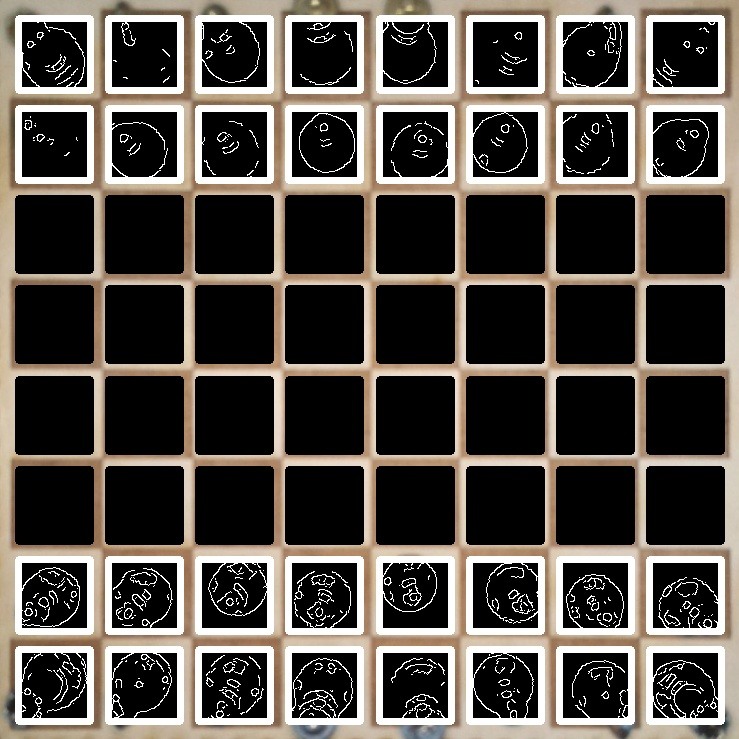
\includegraphics[width=\linewidth]{Images/PieceDetection.jpg}
	\caption{Full Board Piece Detection}
	\label{piece detection}
\end{figure}

All the single square images are superimposed on the board locations they were taken from, with a border added to show whether the square is occupied (the edge count of the square exceeds the comparison threshold) or not. White borders denote an occupied square, no borders denote an empty square.

\vspace{12pt}

\subsubsection{Color Detection}
\label{ColorDetection}
After all the squares have had edge detection run on them to determine if they are occupied, the last piece of information needed to determine the state of the chessboard is the color of each piece.

As can be seen in prior figures, the chess pieces used for this project were silver and gold, these represent white and black respectively. To keep the terminology of sides consistent with standard chess piece nomenclature, pieces will be refered to as white or black, white refers to a silver piece, black refers to a gold piece.

To speed up the processing of each frame, the color detection function is only run on squares that are occupied.

To isolate the chess piece itself, a circular mask is used to only evaluate the color of the pixels inside the edges found in the piece detection function. The position of this mask is determined by calculating the average location of each edge, this centroid is used as the center coordinate of the circular mask.

To determine the radius of the mask, the standard deviation of the Canny edge detection output is computed, this value is then scaled by 135\% and used as the radius of the circular mask.

Once the pixels inside the chess piece have been isolated, the color of the piece is determined by converting the image from RGB to HSV. This makes it much easier to represent the color with a single number, as isolating the first layer of the image gives the hue of the pixel. Figure \ref{color zoomed} shows the hue layer of Figure \ref{piece zoomed} when masked using the edges shown in Figure \ref{piece detection zoomed} and labeled with the calculated color.

\begin{figure}[!ht]
	\centering
	
\includegraphics[width=\linewidth]{Images/ColorDetection340Zoomed.jpg}
	\caption{Single Square Color Detection}
	\label{color zoomed}
\end{figure}

Determining whether a given piece is silver or gold is done by computing the average and standard deviation hue values of each pixel inside the mask. The standard deviation is then subtracted from the average pixel hue as an offset to exaggerate the difference between colors. As can be seen in Figure \ref{color}, a collection of all the color detection images of a chessboard with labeled colors and final offset hue, the white pieces are much more varied and splotchy when compared to the black pieces. In addition to lowering the average hue value of the piece, these dark section also make the standard deviation of the hue much larger. Thus, since the average hue of the white pixels are lower than the average value of the black pixels, and the standard deviation of white hues is larger than the standard deviation of black pixels, by subtracting the standard deviation from the average, the final offset hue values are even further separated.

\begin{figure}[!ht]
	\centering
	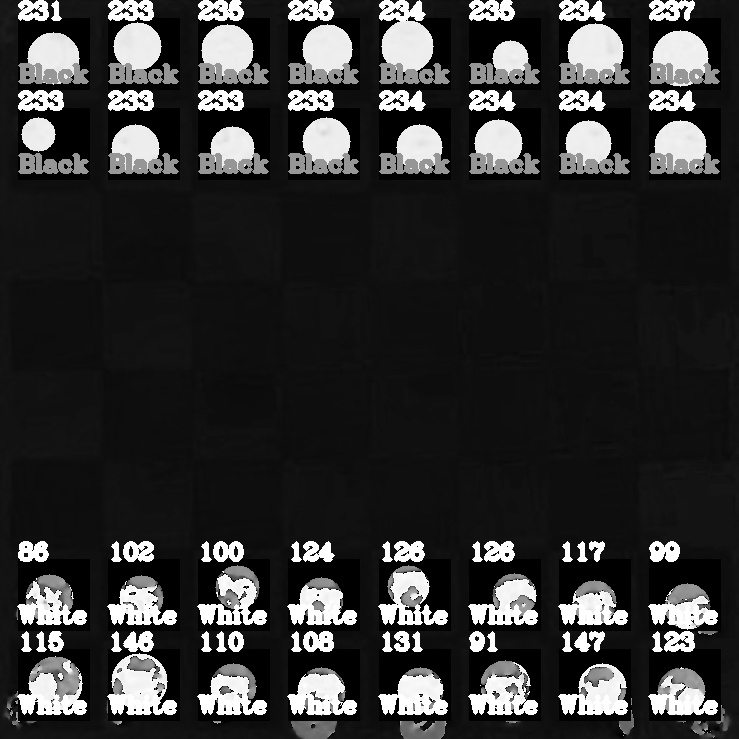
\includegraphics[width=\linewidth]{Images/ColorDetection.jpg}
	\caption{Color Detection}
	\label{color}
\end{figure}

Finally, to sort and classify each piece based on the final offset hue value, the hue values of each piece are sorted, and the lowest are classified as white. To determine how many of each color there should be on the board, the number of each color piece is tracked throughout the match. To start the game, there are always 16 of each color. Since white always moves first, we know the first move will be by white, the second by black, the third by white, and so on. If the total number of pieces counted in the piece detection function is lower than the previous number, we know a piece was captured, and by checking which side it was to move, one can determine the color of the piece that was captured.

For example, if it is black's turn to move and a frame is read that only has 31 pieces in it, then black just captured a white piece, and now 16 black pieces are on the board and 15 white pieces are on the board.

The classified output is then output as an 8x8 array, each value representing a square of the chessboard. A 0 value denotes an empty square, a 1 means the square is occupied by a black piece, and a 2 means the square is occupied by a white piece.

\vspace{12pt}

\subsection{Parsing Detected Moves}
\label{MoveParsing}
After all image processing has been done, the first step in determining what move was made is to determine if any move was made. This can be done simply by comparing the color array for the current frame with the color array of the last frame. If they are equal, than no move was made. Any differences mean a move was made. To measure how many differences there are between arrays, the old array is subtracted from the new array to get an array of differences. The number of non-zero values in this difference array are the number of squares that changed from occupied to empty, empty to occupied, or swapped colors.

The move notation used in this project is Universal Chess Interface (UCI), a notation designed for chess programs on computers. A move is represented by the square the piece leaves, and the square the piece enters. Thus, white advancing their king's pawn is noted as "e2e4".

To determine what type of move was made, the number of differences between the current and past arrays are counted. Simply as a result of how chess moves are made, there can only be 2-4 differences.

\subsubsection{4 Squares Changed}
The only case when the status of 4 squares are changed in one move is when castling, to determine who castled and on which side, one can simply check which corner the moves take place in, and output the corresponding UCI notation for that castling move.

\subsubsection{3 Squares Changed}
The only move where 3 squares change is when a pawn captures another pawn en passant. This means capturing a pawn that is next to yours by passing it and moving into the square behind it. This means the square the capturing pawn was on, and the square it moves to, and the square the captured pawn was on all change, resulting in a total of 3 squares changing.

To get the uci notation of the en passant capture, whichever non-zero value of the difference array appears least is removed. Since the captured piece only appears in one square in the old array, and the capturing piece appears in one square in the old array and a different square in the new array, the captured pawn is effectively removed from consideration. Then, the altered difference array is passed onto the function dealing with difference arrays of 2 non-zero values.

\subsubsection{2 Squares Changed}
Most common moves result in only 2 squares being changed, this happens when one piece moves into an empty square or during normal captures.

Since UCI notation only requires the origin and destination squares to characterize a move, all that is required to compute the move notation given which side is making a move, which squares changed, and the current and previous board layouts is to find the piece of the current colors turn that moved. To do this, one can take the location of the two non-zero elements of the difference array, and check the value of each element in the same location in the old array. The element in the old array that is the same color as the side making a move is the piece in the origin square, and the other non-zero element of the difference array has to be the destination square.

\subsection{Move Recommendation}
\label{MoveRec}
Once the uci move notation is computed, it is send to a board object created using the python chess library that tracks the current layout of board as well as the past history of the game. This board object is then sent to a chess engine, which uses it to compute which move is best for whichever side is up.

\section{Conclusions}
%This is the most important section of the report. Here you should state if your work fulfilled the objectives or not. If it did, you need to discuss how it is demonstrated in this report that this actually happened. If it did not, then you need to say the reasons why and what should be done to fulfill with the objectives (not excuses, the discussion should be technical).  
This chessboard meets the objectives stated in this report: it is able to continuously track chess pieces throughout a chess match in order to always know the layout of the pieces, and use that layout to suggest moves to the user, or play against a computer opponent.
The tracking works by locating the chessboard in the frame of the image taken by the camera using Apriltags as described in Section \ref{ApriltagDetection}, then testing to make sure no objects cross the border of the chessboard to be able to obscure the view of each piece as described in \ref{KnotDetection}, then dividing the chessboard into each individual square and running Canny edge detection to determine whether the square is occupied as described in Section \ref{PieceDetection}. This information is then used to inform the color detection function described in Section \ref{ColorDetection} that determines the color of each piece, which is then fed to the move parsing function described in Section \ref{MoveParsing} that computes which move was made based on the change in the layout of the chessboard. This move is then sent to a chess engine as documented in Section \ref{MoveRec}.

\section{Recommendations}
To save money in producing the product, the plastic parts should be made from injection molding instead of 3D printing, this allows for faster, more repeatable production, and is cheaper than buying thermoplastic filament in bulk. In addition, the ATMega328p microcontroller should be programmed in the factory in order to reduce time and manpower needed to program them on the board.
The camera should be switched from a PiCamera to a USB camera to be more portable across devices as well as reduce the cost of components.

This device could be sold as a training tool for chess players, it is easy to add a chess engine that is capable of beating even the best human players.

As this is a complex system designed and produced in a short amount of time, there are always many aspects that could be improved.
The camera image could be improved by correcting for lens distortion and the fisheye effect. The knot detection is a little distorted and doesn't always match the template near the edges of the board. In addition, not enough effort was put into adapting the settings of the camera to get the best quality image for this project.

Images of each square that has a piece on it should be saved to build up a database of correctly labeled pieces in order to train a machine learning algorithm to recognize piece types so promoted pieces can be automatically recognized. Right now, promoted pieces are automatically assumed to be promoted to a queen, but there are some situations where a player might choose to promote a pawn to a different piece.

Mechanical actuators can be added to allow the computer to move pieces automatically without user input.

The board orientation should be determined on first image instead of assuming the black pieces will be on the left and white pieces on the right.

The color determination settings should automatically work with any color.

The LED ring around the camera should adapt to changes in lighting in order to get the best piece and color detection.

% if have a single appendix:
%\appendix[Proof of the Zonklar Equations]
% or
%\appendix  % for no appendix heading
% do not use \section anymore after \appendix, only \section*
% is possibly needed

% use appendices with more than one appendix
% then use \section to start each appendix
% you must declare a \section before using any
% \subsection or using \label (\appendices by itself
% starts a section numbered zero.)
%


\appendices
\section{Code Repository}
\label{Github repo}
The code for this project can be found here: \url{https://github.com/blemay360/Chessboard}

% you can choose not to have a title for an appendix
% if you want by leaving the argument blank
%\section{}
%Appendix two text goes here.

% Can use something like this to put references on a page
% by themselves when using endfloat and the captionsoff option.
\ifCLASSOPTIONcaptionsoff
  \newpage
\fi



% trigger a \newpage just before the given reference
% number - used to balance the columns on the last page
% adjust value as needed - may need to be readjusted if
% the document is modified later
%\IEEEtriggeratref{8}
% The "triggered" command can be changed if desired:
%\IEEEtriggercmd{\enlargethispage{-5in}}

% references section

\printbibliography

% that's all folks
\end{document}


